% REMEMBER: Write the thesis from the view of the reader. How would I like to READ the thesis?
% WHY -> WHAT -> HOW structure

% FROM APPROACH:
% - Before starting a test case, the project is loaded to make sure that every test starts with the same program state
%     - If this would not be done, it would be very hard to test programs that don't do proper initialization
%     - Tests would depend on the state the previous test leaves the program in
%     $\rightarrow$ Very inconsistent, therefore desirable to load the program before each test

%         - This work will explore automatic generation of input for Scratch programs
%         - Input can be generated randomly
%         - Static analysis can be used to detect the input events the program recognizes and to give the program inputs
%         - A combination of both will be used for this work

\chapter{Implementation}

TODO: keyword "automation"

- This section shows a implementation of a testing utility for Scratch
- Uses the approach described above
- Implemented in JavaScript (ES6) for compatibility with Scratch 3.0, which is implemented in JavaScript

\section {Scratch 3.0 Implementation Details}

Scratch's interpreter sequentializes the execution.
This is necessary for the single-threaded JavaScript environment Scratch is run in.
This means that no race-conditions can occur on a language level.

\section{General Design}

- TODO explain Scratch's design?
- TODO explain why it's possible to execute code before and after Scratch's step without interfering with the Scratch program

- Tests are written in JavaScript
- Usually one test is a function of a .js file

- Does not change the virtual machine in any way
    $\rightarrow$ designed so it can be used with any instance of the Scratch virtual machine
    $\rightarrow$ same version of Whisker can be used with different versions of the Scratch virtual machine
    $\rightarrow$ even something like a browser addon for the original Scratch page would be possible

- Whisker is designed to be a layer between test code and the scratch virtual machine
- Allows to interact with the VM in a test-friendly way
- The main class VM Wrapper and its components make up a wrapper around the scratch virtual machine,
  which offers extra functionality for testing
- Test Driver offers a user-friendly interface between the test code and the VM Wrapper
- Test uses Test Driver to simulate input, get information about sprites

- Test Driver could be acquired through a helper method or passed to the test method
- Up to the testing framework to provide the test driver
- The examples in this chapter will refer to the test driver with the variable \texttt{t}

\begin{listing}[ht]
    \centering
    \begin{minipage}[t]{.45\textwidth}
        \begin{javascriptcode}
            async function test (t) {
                ...
            }
        \end{javascriptcode}
        \vspace{-\bigskipamount}
        Getting the test driver as a parameter to the test function
    \end{minipage}
    ~
    \begin{minipage}[t]{.45\textwidth}
        \begin{javascriptcode}
            async function test () {
                const t = acquireTestDriver();
            }
        \end{javascriptcode}
        \vspace{-\bigskipamount}
        Getting the test driver through some helper method
    \end{minipage}
    \caption{Examples of how to acquire the test driver}
    \label{fig:examples_of_how_to_acquire_the_test_driver}
\end{listing}

=== Limitations
- Scratch depends on the renderer
    - Some functionality of the Scratch virtual machine depends on the renderer
    - Headless tests are impossible without restricting the Scratch program to a subset of available blocks
- Therefore Whisker assumes the VM is always run with a renderer in place

\begin{figure}[ht]
    \centering
    \tikzset{>=latex,
             label/.style={draw=none, text width=5.3cm, minimum height=0.5cm, text centered},
               box/.style={draw,      text width=2.5cm, minimum height=0.7cm, text centered, rounded corners},
                 h/.style={fill=blue!10}}

    \begin{tikzpicture}
        \node[box]   at ( 0.0,  3.0) (testcode)      {Test Code};
        \node[box]   at ( 0.0,  1.5) (testdriver)    {Test Driver};
        \node[label] at ( 0.0,  0.0) (vmwrapper)     {VM Wrapper};
        \node[box]   at (-1.4, -0.7) (sprites)       {Sprites};
        \node[box]   at (-1.4, -1.6) (inputs)        {Inputs};
        \node[box]   at ( 1.5, -0.7) (callbacks)     {Callbacks};
        \node[box]   at ( 1.5, -1.6) (constraints)   {Constraints};
        \node[box]   at (-2.0, -3.2) (scratchvm)     {Scratch VM};
        \node[box]   at ( 2.2, -3.2) (scratchrender) {Renderer};

        \begin{scope}[on background layer]
            \node[draw, h, rounded corners, fit=(vmwrapper)(sprites)(inputs)(callbacks)(constraints)] (container) {};
        \end{scope}

        \foreach \pp/\pf/\pt in {--/testcode/testdriver,
                                 --/testdriver/container,
                                 --/container/scratchvm,
                                 --/container/scratchrender,
                                 --/scratchvm/scratchrender}
        \draw[shorten >= 2pt, ->] (\pf) \pp (\pt);

        % \draw[shorten >= 2pt, rounded corners, dashed, ->]
        %        (constraints)
        %     -- ( 3.5, -1.6)
        %     -- ( 3.5,  3.0)
        %     -- (testcode);
        % \draw[dashed, -] (callbacks) -- ( 3.5, -0.7);
    \end{tikzpicture}

    \caption{Components of Whisker}
    \label{fig:components_of_whisker}
\end{figure}

\section{The Step Loop}

- The core of the Scratch virtual machine is a step-function, which is called at a constant interval (using JavaScript's \texttt{setInterval()})
- Interval of 30 times / second for Scratch 2.0, 60 times / second for Scratch 3.0
- The function executes the program until a time limit is reached and then redraws the scene
- If some visual change occurs in the project, the program execution is stopped earlier and the scene is rendered

\begin{listing}[ht]
    \centering
    \begin{javascriptcode}
        STEP_TIME = 1000 / STEPS_PER_SECOND;
        WORK_TIME = 0.75 * STEP_TIME;

        while (running &&
               timeElapsed < WORK_TIME &&
               !redrawRequested) {
            for (thread of threads) {
                stepThread(thread);
            }
        }

        renderer.draw();
    \end{javascriptcode}
    \vspace{-\bigskipamount}
    \caption{Simplified Scratch Step Procedure}
    \label{fig:simplified_scratch_step_procedure}
\end{listing}

- Instead of executing the step function via interval, Whisker executes its own step loop, which calls Scratch's step function
- Before and after the step of the Scratch program, test code is run, registered inputs are performed and sprite objects are updated

- This should either not affect the Scratch program, or only affect it minimally
    - Renderer might not need to use the entire allocated rendering time
    - If something changes in a Scratch program, usually a sprite moves $\rightarrow$ Scratch will only use a fraction of the entire allocated work time in most cases
    - Scratch uses real time to track wait times $\rightarrow$ not affected much by a step that takes longer that normally

=== Scratch programs depend on real time
- Possible problem: additional computations could cause the program to run slower
- Scratch blocks that involve timings, like "wait" or "say for secs" use real time to delay execution
$\rightarrow$ If the additional computations take too long, they could influence the program

\begin{figure}[ht]
    \centering
    \tikzset{>=latex,
             box/.style={draw, text width=4.3cm, minimum height=0.7cm, text centered, rounded corners},
             num/.style={draw, circle, inner sep=0.6mm, text centered},
               h/.style={fill=blue!10}}

    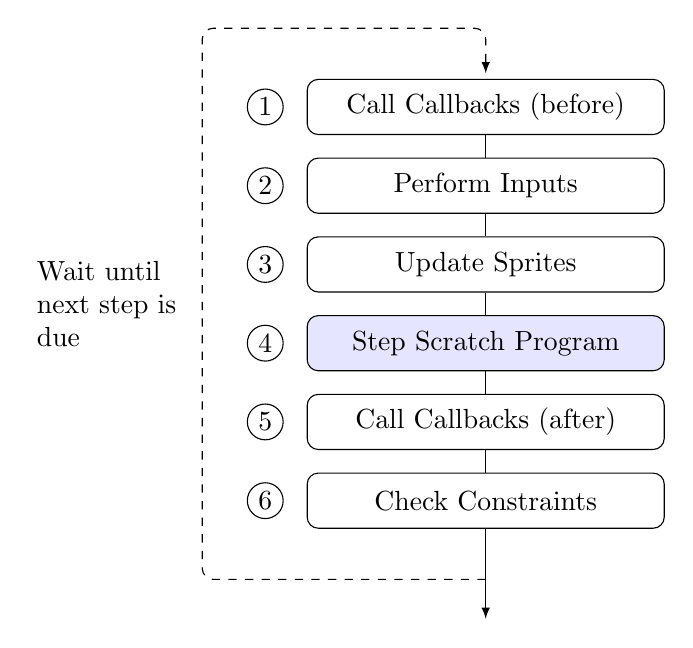
\begin{tikzpicture}
        \node[box]    at ( 0.2,  5.0) (callbacksbefore) {Call Callbacks (before)};
        \node[box]    at ( 0.2,  4.0) (inputs)          {Perform Inputs};
        \node[box]    at ( 0.2,  3.0) (sprites)         {Update Sprites};
        \node[box, h] at ( 0.2,  2.0) (step)            {Step Scratch Program};
        \node[box]    at ( 0.2,  1.0) (callbacksafter)  {Call Callbacks (after)};
        \node[box]    at ( 0.2,  0.0) (constraints)     {Check Constraints};

        \node[text width=2cm] at (-4.5, 2.5) (wait)  {Wait until next step is due};

        \node[num] at (-2.6,  5.0) (one)   {1};
        \node[num] at (-2.6,  4.0) (two)   {2};
        \node[num] at (-2.6,  3.0) (three) {3};
        \node[num] at (-2.6,  2.0) (four)  {4};
        \node[num] at (-2.6,  1.0) (five)  {5};
        \node[num] at (-2.6,  0.0) (six)   {6};

        \draw[->]
               (callbacksbefore)
            -- (inputs)
            -- (sprites)
            -- (step)
            -- (callbacksafter)
            -- (constraints)
            -- ( 0.2, -1.5);

        \draw[shorten >= 2pt, rounded corners, dashed, ->]
               ( 0.2, -1.0)
            -- (-3.4, -1.0)
            -- (-3.4,  6.0)
            -- ( 0.2,  6.0)
            -- (callbacksbefore);
    \end{tikzpicture}

    \caption{Whisker Step Procedure}
    \label{fig:whisker_step_procedure}
\end{figure}

\section{The Basic Testing Functionality}

=== WM Wrapper
- Control the execution of the scratch program
- Run the program until a certain amount of time has passed or a condition has been met
- Get the time elapsed since the start of the test or the start of the last run
- Cancel a run
- Uses JavaScript's Promise API to wait until a run is finished

\begin{listing}[ht]
    \centering
    \begin{javascriptcode}
        await t.runForTime(500);
        await t.runUntil(() => !t.projectRunning(), 1000);
        t.assert.ok(t.getTotalTimeElapsed() < 1000);
    \end{javascriptcode}
    \vspace{-\bigskipamount}
    \caption{Example code for the VM Wrapper}
    \label{fig:example_code_for_the_vm_wrapper}
\end{listing}

=== Sprites
- Sprite is not the same as sprite in Scratch VM
    - Explain distinguishes between sprites and targets / rendered targets
    - Sprite contains the blocks, graphics (costumes), etc.
    - Target / rendered target is an instance of the sprite
    - Whisker sees every rendered target as a sprite
    - The original target of a Scratch sprite as well as its clones are each an instance of a ''sprites''
    - TODO: explain clones here

- Sprites work by wrapping around the original
- If some getter of the sprite is called, the actual value is retrieved from the original target
- Most properties are implemented as JavaScript getters $\rightarrow$ look like properties of Whisker's sprite object

- Information about sprites and variables
- Gives the information that the test uses
- Does not allow to manipulate sprites and variables
- Contains ''old'' value for every fitting property
    - Saves the value from the last step
    - Useful for constraints (see later)
    - Initialized with the present value
- Sprites are only tracked once they are retrieved via one of the getter method
- Helps, for example, with programs that spawn a lot of clones (could pose a performance problem otherwise)


\begin{listing}[ht]
    \centering
    \begin{javascriptcode}
        const sprite = t.getSprite('Sprite1');
        const variable = sprite.getVariable('Variable1');
        const sprites = t.getSprites(s => s.x > 100);

        t.assert.equal(sprite.x, 100);
        t.assert.equal(sprite.old.x, 100);
        t.assert.equal(variable.value, 5);
    \end{javascriptcode}
    \vspace{-\bigskipamount}
    \caption{Example code for Sprites}
    \label{fig:example_code_for_sprites}
\end{listing}

=== Inputs
- INPUTS ARE SIMULATED ON THE VM, NO ACTIONS ARE SIMULATED ON THE OS LEVEL OR ANYTHING

- Simulate inputs on the program
- Can be registered to be called after a certain amount of time or be executed immediately
- Registering a Input with 0 delay is different from executing it immediately
=== Kinds of Input
- At the moment: only mouse and keyboard input
- Keyboard:
    - Press a key
    - Release a key
    - Toggle a key
    - Press / release a key for a certain duration
- Mouse (only left mouse button):
    - move cursor to position
    - move cursor to sprite (+offset)
    - press mouse button
    - release mouse button
    - toggle mouse button
    - Press / release mouse button for a certain duration

\begin{listing}[ht]
    \centering
    \begin{javascriptcode}
        t.inputImmediate({
            device: 'keyboard',
            key: 'right arrow',
            isDown: true
        });

        const mouseInput = t.addInput(1000, {
            device: 'mouse',
            x: 100,
            y: 0,
            isDown: true,
            duration: 500
        });

        t.assert.ok(t.isKeyDown('right arrow'));
        t.removeInput(mouseInput);
        t.addInput(mouseInput);
    \end{javascriptcode}
    \vspace{-\bigskipamount}
    \caption{Example code for Random Inputs}
    \label{fig:example_code_for_random_inputs}
\end{listing}

=== Random Inputs
- Provides a simple way to perform inputs randomly
- Way of testing the program without deliberately controlling the inputs
- In a set time interval (at the next step), an input is randomly selected from a pool of registered random inputs

- You  can register inputs for the random pool, or let Whisker choose inputs based on the blocks used in the program
- Random inputs can be detected through simple static analysis
$\rightarrow$ Blocks that take inputs and their options are analyzed

- TODO table of detected blocks and resulting inputs ?

\begin{listing}[ht]
    \centering
    \begin{javascriptcode}
        t.setRandomInputInterval(150);
        t.registerRandomInputs([
            {
                device: 'keyboard',
                key: 'left arrow',
                duration: [50, 100]
            },
            {
                device: 'keyboard',
                key: 'right arrow',
                duration: [50, 100]
            }
        ]);
        t.detectRandomInputs();
    \end{javascriptcode}
    \vspace{-\bigskipamount}
    \caption{Example code for Inputs}
    \label{fig:example_code_for_inputs}
\end{listing}

=== Callbacks
- Register callbacks that are called after every step
- Can be registered to run at two positions in the step cycle (see diagram later)
- Purpose:
    - Information Tracking:
        - Track events
        - e.g how many times a sprite touches some other sprite
              or how long a sprite is invisible, etc.
    - Inputs:
        - Allows performing conditional inputs
        - Control the program like a player would
        - e.g. follow a sprite with the mouse cursor

\begin{listing}[ht]
    \centering
    \begin{javascriptcode}
        const sprite = t.getSprite('Sprite1');

        const callback = t.addCallback(() => {
            t.inputImmediate({
                device: 'mouse',
                x: sprite.x,
                y: sprite.y
            });
        });

        await t.runForTime(1000);

        callback.disable();
        callback.enable();
    \end{javascriptcode}
    \vspace{-\bigskipamount}
    \caption{Example code for Callbacks}
    \label{fig:example_code_for_callbacks}
\end{listing}


=== Constraints
- Describe conditions that must always hold
- Failed constraints can be configured to fail the test, stop the current program run (\texttt{run...()}), or do nothing
- Can be used to perform checks like "sprite xy is always visible when sprite yz is visible"
- Implemented as callbacks that execute assertions
    - Advantages:
        - Concise syntax
        - Multiple assertions per constraint possible
        - Assertion messages can be used to describe the constraint failure
    - Disadvantages:
        - Assertion methods have to be efficient, e.g. if assertion message is constructed every time it could be too slow
        - Need to catch exceptions if constraints should not fail the test
- Can separate assertions from the program execution
    - Define constraints for tested properties, then use whatever input (deliberate / random / manual)
    - Problem: most constraints still hold if the tested property is not implemented at all
        - e.g. constraint that checks that a sprite never moves left will hold if the sprite doesn't move at all

\begin{listing}[ht]
    \centering
    \begin{javascriptcode}
        const sprite = t.getSprite('Sprite1');

        t.onConstraintFailure('fail');

        const constraint = t.addConstraint(() => {
            t.assert.ok(sprite.x >= sprite.old.x);
        });

        await t.runForTime(1000);

        constraint.disable();
    \end{javascriptcode}
    \vspace{-\bigskipamount}
    \caption{Example code for Constraints}
    \label{fig:example_code_for_constraints}
\end{listing}

\section{Automated Test Input Generation}

\section{Coverage Measurement}
- Whisker can measure simple statement coverage
- Project wide and for single sprites / the stage

- Only measures blocks that are part of a script / connected to a hat (this includes procedure definitions)
- Other blocks are obviously not reachable

- Useful to detect if a project has been properly captured by a test
    - If coverage is low, there is a problem with the test or project
    - Or the project contains unnecessary code

- Initialized by traversing the scripts and noting each block id of the blocks in a project
- Coverage is simply measured by tracking which block ids are put on top of the stack of the threads in the Scratch virtual machine

\section{Running Tests}
\label{sec:running_tests}
- Whisker comes with an optional testing framework
- Include a sample test report?

=== Seeing test output, interactive tests
- Users will want to see the program's output while it is run
    - to check if the tests run correctly, to check if the program runs correctly
    - Difficult to determine a problem with the project from just textual test reports
    - Tests without showing output are not very useful in such an interactive environment
$\rightarrow$ Has to be able to run in a interactive environment
    - Web GUI, which can be run by any modern browser
    - Allows users to run individual tests on the project and see the program execution

=== Batch Testing of Projects
- Some tests for Scratch projects can take a long time because projects run in real time
    - raises the need to test scratch programs in parallel
    - Scratch depends on the renderer
        - Some functionality of the Scratch virtual machine depends on the renderer
        - Headless tests are impossible without restricting the Scratch program to a subset of available blocks
$\rightarrow$ Web GUI has the option to run tests on multiple projects sequentially, but this might still take a long time depending on the project and the test suite
$\rightarrow$ Electron
    - Running tests in multiple processes could circumvent the problem
    - Electron provides a renderer that can be used to render the Scratch output to
    - Spawns multiple processes which open a window each, one project is tested in each window
